\documentclass[12pt,a4paper,titlepage]{scrreprt}
\usepackage{url}
\usepackage{fullpage}
\usepackage{amsmath,amssymb}
\usepackage{graphics,graphicx,wrapfig,float,epsfig,subfigure,sidecap}
\usepackage{url}
\usepackage{svg}
\usepackage{graphicx}
\usepackage{apacite}
\usepackage{setspace}
\usepackage[margin=0.45in]{geometry}

\usepackage{color}

\begin{document}

    \title{PsychoCoffee}
    \subtitle{Open, Robust, Experimenter-Friendly Data Collection via the World Wide Web}
    \date{\small{{rtibbles}@ucsd.edu}}
    \author{{\bf Richard Tibbles} \\ \\
                \small{University of California, San Diego} \\
                \small{Department of Cognitive Science} \\
                \small{Center for Human Development}}
    \maketitle
\newpage

\tableofcontents

\newpage

\chapter{Introduction}
    
    The basic question of the Psychological Sciences is to understand the function and instantiation of the human mind. The investigation of such phenomena thus far in the history of Science has been highly focused on the minds of individuals in very particular social contexts. In contrast to the physical sciences, where the particular spatial location of experiments is assumed to have no bearing on the fundamental laws being investigated (and more strongly, were it to do so, these would not be 'fundamental' laws as we understand them), it is at the very least an open question in psychological sciences the extent to which the social context affects the phenomena under investigation. In addition to social context, the population of minds in which psychological investigations are generally undertaken is also considerably limited as compared to the broad swathe of humanity.
    In addition to a bias in the sampling of minds, and the contexts of minds, there is insufficient replication of positive results in the literature. Replication is a time consuming process, requiring an experimenter to recreate an experiment conducted by a colleague. However, if there is no obvious extension of the experiment, the incentive for this replication will be very low, as no original results can be further tested in the replication of an older experiment. In addition, the original positive result may be very closely tied to certain features of the experimental setup - while it is desirable that results be robustly replicable, it is also of interest to discover the relevant reasons why results do not replicate. Finally, direct replication, whereby the repetition of the experiment in all relevant details is undertaken in a different laboratory, by different researchers, is incredibly rarely done, and is not incentivized.
    In order to provide a tool to contribute one part of a range of possible solutions to the above problems, a framework for online experimental testing is proposed. An online experimental system has the advantage of being able to reach a wider range of potential participants, allow for the gathering of larger datasets with lower experimenter effort, and the rapid replication of existing experiments, through the sharing of experimental materials. While similar systems are already in development and use, they lack several key features to help tackle the problems outlined above. To this end, the proposed system, PsychoCoffee, will be: open source, integrate features and defaults for open sharing and alteration of experimental code, and scaffold creation of experiments with a graphical user interface.
    The system will be open source in order to allow for inspection of the source code to verify, modify, and enhance the system for particular experimental needs. Developing software as open source is in line with the Scientific demand for clarity and disclosure of experimental methods. Without the ability to inspect the source code of experiments and the experimental framework, claims about the system are not amenable to independent verification.
    Leveraging existing mechanisms for sharing and distributing code will allow experimenters to rapidly replicate, modify, and extend colleague's experiments, in order to test the range of replication of experiments, and to investigate additional aspects of phenomena. Finally, the use of a graphical user interface to define the elements and control flow of an experiment will allow broader and more efficient participation in experimental design and creation, in a time when programming is still a much sought after skill in Social Science laboratories.

\newpage

\chapter{Related Work}
\section{Open Science}
[Section on the confluence of Open Science and Open Source software, and how Open Science demands Open Source analysis and experimental software.]
\section{Replicability and Generalizability}
Although there have been concerns for nearly forty years\cite{greenwald_consequences_1975} about the truth and generalizability of published research in Psychology, the coining of the \textit{replicability crisis}\cite{pashler_editors_2012} seems to have catalyzed action on behalf of at least some actors in the field. The root of much of the current concern was first named as the file drawer problem in the last century\cite{rosenthal_file_1979}. The initial problem is simply articulated - in the extreme case, the bias for publishing positive results means that at an alpha criterion for significance of 0.05, a researcher's file drawer could contain nineteen failed experiments that failed to show statistical significance for every one experiment that showed statistical significance, the net result being that the evidence for the effect supported by the one published study is no better than chance.
To compound the file drawer effect, verification of positive results is frequently via conceptual, rather than direct replication\cite{pashler_is_2012}. This has the result that verifications can be taken as evidentially supportive of the original publication, whereas falsifications can be dismissed as operationally different, and hence uninformative to the evidential basis of the original result. In addition, surveys of the literature have found that very few direct replications of positive research findings occur\cite{makel_replications_2012} - in this way, a result that, by chance, was deemed significant can be the basis for bootstrapping an entire research program through conceptual replications based off a single finding that may lack evidential basis.

\subsection{Meta-Analyses of Reported P-Values}
The extent of the problems in the current literature can be quantified using meta-analytic methods. While the methods themselves cannot, of course, indicate the truth or falsehood of a particular study finding, analysis of the distributions of statistical values can help to highligh research practices that will tend to inflate the statistical significance of a phenomenon\cite{john_measuring_2012}. These practices include: unreported exploratory analyses (doing analyses until a significant p-value is found, but only reporting the significant analyses), stopping the experiment when a significant result is found, and removing outliers after initial analyses have been run - these will all increase the effective alpha criterion for significance of the effect reported, as more comparisons have been conducted than have been reported. These strategies will all tend to exacerbate the effect of the file drawer problem, creating even more studies that are likely to be false positives\cite{bakker_rules_2012}.
Fortunately, there is some hope for detecting these methodological biases through meta-analytic statistical tests of the distribution of p-values, in an attempt to highlight possible instances of \textit{p-hacking}\cite{simonsohn_p-curve:_2013}. \textit{P-hacking} is used to describe the above practices (and others) that might result in the inflation of the number of significant p-values in the literature.
To detect \textit{p-hacking}, it must be first recognized that there will be a highly biased sample of p-values in the literature, due to publication biases for positive effects. However, a null effect that has been reported without \textit{p-hacking} will have a distribution of p-values proportional to the p-values themselves - that is a p-value of 0.045 would have a probability of 0.045 of occurring, this can then be rescaled to take into account the bias towards reporting results with p-values of less than 0.05. A real effect, however, will have a distribution of p-values that is skewed towards lower p-values, as a real effect will more frequently appear to be distributed differently from the null at greater than the alpha criterion for chance.
By contrast, reported p-values in the literature that are the result of \textit{p-hacking} will have a skew towards lower p-values, as their criterion for appearing in the literature is simply being less than the alpha criterion of 0.05. Under conditions of \textit{p-hacking}, the process will halt as soon as a result just less than 0.05 is reached, and so the distribution will be skewed towards the upper end. This could have the net result of \textit{p-hacking} on real effects resulting in an appearance of null results - the only hope is that there are sufficient sufficiently powered studies in the literature to counteract any results of \textit{p-hacking} for real effects.

\subsection{Endemic Lack of Replication}

A crude but effective survey of the existing literature searched for articles that contained the search term "replica*"\cite{makel_replications_2012}. In order to assess the correlation of the positive match of the search term with actual replication of experimental results (rather than simply proposing replication or some other phrase that would match), a sub-sample of 500 articles was inspected by the researchers. 68\% of these were reported as actual replications (whether conceptual or direct), and this scaling was used to attenuate the reported results for percentage of articles that were replications.
After this scaling, 1.07\% of all articles were found to be replications, with a trend over time towards a slight increase in replications in the recent past. However, the trend for replications was towards conceptual, rather than direct replications, over time, and towards authors of the studies being replicated doing the replications. Independent, and more generalizable replication of experimental results appears to have reduced.
While the majority of replications were successful, there was a significant difference in replication success rate if the replication was conducted by someone other than the original study's authors.
One encouraging finding of the study is that the median citation count for the replications was 17, while significantly lower than the median citation count of the articles being replicated (64.5), it was significantly higher than the median citation count for the journals surveyed. This suggests that to some extent the replication of results is valued by the scientific community.
\subsection{Generalizability of Results}
\begin{quote}Some say that psychological science is based on research with rats, the mentally disturbed, and college students. We study rats because they can be controlled, the disturbed because they need help, and college students because they are available.\cite{birnbaum_psychological_2000}
\end{quote}
While it is obvious to practising researchers that most participant pools are composed of very limited populations\cite{buchanan_using_1999,birnbaum_psychological_2000,kraut_psychological_2004,birnbaum_human_2004,buhrmester_amazons_2011}, the classification of the majority of behavioural experiment participants as Western, Educated, Industrialised, Rich, from Developed countries (or WEIRD), and the highlighting of disparities in performance on canonical psychological tasks between these participants and a broader selection of humanity \cite{henrich_beyond_2010} has helped to bring the limitations of these populations into sharp focus. While the strong thesis of Henrich et al. that the most frequent participants in behavioural experiments (i.e. American undergraduate students) are outliers in human psychology goes too far\cite{bennis_weirdness_2010}, it is generally acceptable at least that claims of universality of behavioural phenomena from this sample go too far\cite{baumard_weird_2010,ceci_weird_2010,konecni_responsible_2010}.
\subsection{Improving Replication and Generalization}
While statistical meta-analytical techniques can indicate likely instances of methodological issues, to verify or falsify reported effects, both a guarantee of confirmatory research, and direct replication are needed. Several strategies for this have been suggested. Scientists could be incentivized scientists to replicate studies, by offering joint publication with the original study\cite{koole_rewarding_2012}, creating metrics and crowdsourcing replication\cite{nosek_scientific_2012}, creating an open collaborative framework for sharing replication efforts, materials, and results\cite{collaboration_open_2012}, and using undergraduate research projects (both independent research projects, and in project based learning classes) as a means of conducting direct replication\cite{grahe_harnessing_2012,frank_teaching_2012}. Additionally, the open sharing of data, materials, and workflow\cite{giner-sorolla_science_2012,nosek_scientific_2012,miguel_promoting_2014} are all highlighted as ways to open up both the experimental process and experimental results to proper scrutiny and replication. Effort to replicate is also a significant barrier, which the use of online data collection can help to overcome\cite{grahe_harnessing_2012}.
Finally, online experiments can help to broaden the participant pool\cite{gosling_wired_2010} - unfortunately, due to the current global distribution of Internet access, mostly concentrated in industrialized countries, and with the affluent of more rapidly developing ones, opportunities will be restricted to discover behavioural phenomena that are robust across industrialized cultures, and more affluent members of rapidly developing societies.
\section{Online Experiments}
One way, therefore, to broaden the reach of psychological research beyond the participants immediately available in the vicinity of the laboratory is to use Internet based studies to recruit a far broader and heterogeneous population. In early web studies, the lack of widespread Internet penetration led to concerns of repeating the same population difficulties shown in undergraduate recruitment - however, in a range of areas of study, from decision making to social psychology, experiments successfully replicated the results of laboratory based studies, while still attracting a more diverse sample than would ordinarily be the case\cite{krantz_comparing_1997,buchanan_using_1999,birnbaum_decision_2000,mcgraw_integrity_2000,gosling_should_2004,ritter_internet_2004}. Further, the development of this new methodology quickly led to the formulation of best practices to overcome some of the perceived issues of confidentiality, reduced experimental control, multiple submissions, incomplete submissions, dropout, and misunderstanding instructions\cite{reips_web_2000,reips_standards_2002,birnbaum_human_2004}. While it is not always the case that study materials used in laboratory experiments can be used identically online and yield the same results\cite{buchanan_nonequivalence_2005}, the web provides an intermediary point between the laboratory and field studies to test the generalizability of experimental procedures and findings to less controlled contexts. It can also reduce experimenter bias and demand characteristics, and allow for experimental measures between subjects of motivational effects of studies through comparisons of drop out rate\cite{reips_web_2000}, which is less measurable in laboratory experiments due to the pressure from the social context of the experiment, and frequently the desire for class credit.
\subsection{Current Applications}
[Section exploring range of experiments implemented online.]
\subsection{Current Practices}
[Needs more]
Many participants for online experiments are now paid, similarly to many laboratory studies, particularly through the use of crowdsourced labour platforms such as Amazon's Mechanical Turk\cite{buhrmester_amazons_2011,rand_promise_2012,crump_evaluating_2013}. However, other work has relied entirely on voluntary participation, with significant boosts to participation coming from media coverage (and in the case of data gathered through the BBC UK Lab, through cooperation with the BBC television show \textit{Bang Goes the Theory})\cite{owen_putting_2010,germine_is_2012,halberda_number_2012}.
\subsection{Challenges for Online Experiments}
[Needs more]
Very short stimulus presentation times, on the order of 64ms and below, have not been able to be used so far in web based experiments\cite{crump_evaluating_2013}. In addition to thresholding the lower limits for length of stimulus presentation, it is also important to understand the characteristics of different participant devices, and their accuracy with regards reaction time measurements.
\section{Experimental Implementation}
\subsection{Current Practices}
[Needs more - ePrime, Presentation, PsychToolbox, etc.]
The proposed platform, PsychoCoffee, is modelled after another success in open source software for Psychological research - PsychoPy\cite{peirce_psychopypsychophysics_2007,peirce_generating_2008}. PsychoPy is a platform for generating Psychophysical and Psychological experiments. By leveraging a powerful, multipurpose, cross-platform language like Python, PsychoPy allows researchers to develop code that will run in the same way across multiple computers and operating systems. In addition, because the framework itself is Open Source, more technically minded experimenters are able to add new features that they need for their experiments. Using this framework, PsychoPy has achieved the difficult dual task of creating a stable but customizable platform. In addition, due to the focus of the Python language itself on readability of code\cite{_python_????}, experiments coded using PsychoPy are amenable to inspection by other scientists, seeking either to verify, replicate, or extend research findings. As such, PsychoPy goes a long way in assisting Psychology in creating open experiments to increase scrutiny and replication, also, due to the cross-platform (and free) nature of the underlying language, the bar for replication is lowered considerably.
\subsection{Challenges for Implementing Experiments}
Issues still remain, however, as the extra step of sharing experimental code, no matter how readable it naturally is, remains a barrier to openness. In addition, the difficulty of replication in participant recruitment, use of laboratory space, and personnel remains a barrier. To address this, PsychoCoffee will use coffeescript, a readable Python-inspired form of the Javascript programming language to maintain the accessibility of PsychoPy, while creating an experimental platform designed for the Web.
While many Psychology laboratories are already using the Web for experiments, and have created their own frameworks within which to create their experiments\cite{krantz_comparing_1997,germine_is_2012}, no platform is yet available for general purpose programming of online experiments. One program in development is Cognilab\cite{_cognilab_????}, run by a private company startup, with no obvious plans to open source their software. Success of this software would do little to open up the processes of scientific experiments to scrutiny and inspection as required by the foregoing concerns about the state of Psychology.
\section{Supporting Programming}
SCRATCH ETC.
\chapter{Research Questions}
\begin{itemize}
\item How to design a system to support rapid prototyping and development of psychological tasks?
\item How to design an experimental platform to be scalable, robust, and collect reliable experimental data across a range of user devices?
\item How to design a system that encourages open sharing of experimental code and materials, to allow for rapid replication and extension?
\item How precise and accurate can web based sensing deployed through arbitrary devices be?
\item Can the sensor characteristics of such a system be remotely determined through automated tests and user input when compared with data collected in more controlled environments?
\end{itemize}
\chapter{Proposed Research}
\section{System Design}
\subsection{Open Source}

The system will use the existing code versioning tool, git\cite{_git_????}, and the open source code sharing platform github\cite{_github_????}, during the experimental implementation process. This will allow the quick sharing, modification, and extension of experiments created within it. As a default in the system, these materials will be openly licensed, and free to be distributed. Using these existing tools to share experimental code and materials will enhance the capacity to replicate and interrogate the methods used by behavioural science in gathering data\cite{giner-sorolla_science_2012,nosek_scientific_2012,miguel_promoting_2014}. In addition, the use of a versioning system, such as git, allows for modifications and extensions to experiments to be tracked - both across time and across researchers. By examining the task demands across these different changes, and subsequent behavioural measures, researchers can start to collectively define the extent of generalizability of findings, based on the extent of replication given different modifications and extensions.

By leveraging the resources of these existing Open Source tools, experimental code will be freely shared, modifiable, and the differences between different versions of experiments will be readily inspectable using widely used tools.
\subsection{Extensible Framework}
The platform would use a modular approach to stimuli presentation and response capturing. By defining programmatic base classes of stimulus and response, the software can be incrementally developed by the original developers, and later by the broader community, to suit varied experimental needs. 
\subsection{GUI Based Programming}
In addition to creating an open framework, the platform will have a graphical user interface for experiment design, modelled after the PsychoPy Builder (a timeline based view of experimental components that can be manipulated without any knowledge of the underlying Python code), and the MIT Scratch programming language\cite{resnick_scratch:_2009}. This will help to lower a further barrier to replication, allowing the platform to be used in undergraduate replications of existing research findings \cite{frank_teaching_2012}, and also letting those with less programming experience have a scaffolded programming experience to create the flow of their experiments.\\
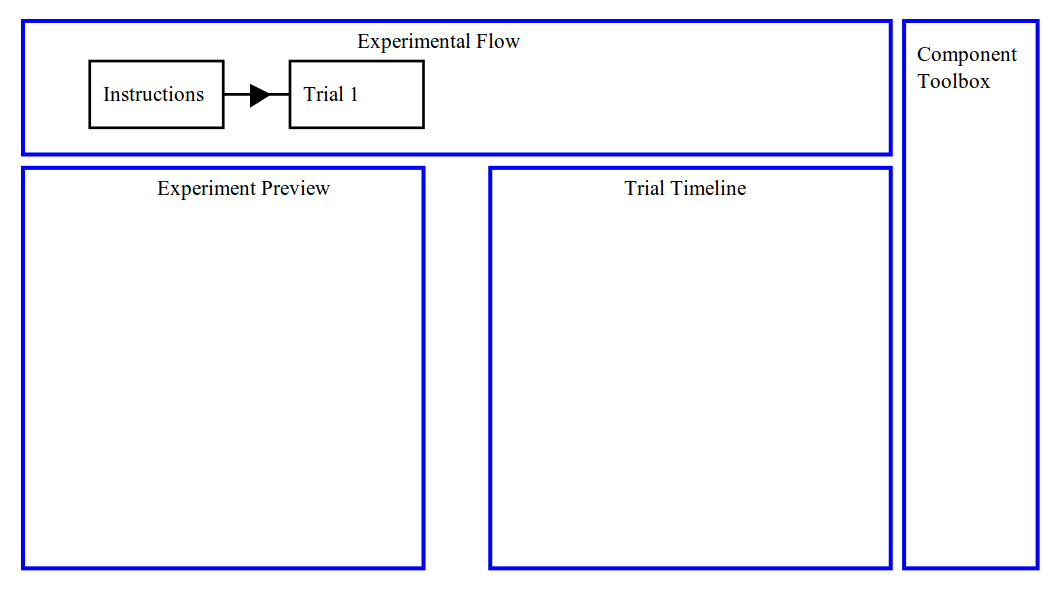
\includegraphics[scale=0.4]{edit_interface}
\section{Problem Finding}
\subsection{User Surveys}
User surveys will be used to gather more in depth information about current practices in the research community around online data collection than is available in literature sources.
\subsection{Participant Observations}
Users using current tools for creating online experiments (such as modifications to Qualtrics, custom programming on Amazon Mechanical Turk, Google Forms, SONA surveys etc.), will be observed in order to understand current pain points in developing online experimental materials.
\section{Prototyping}
\subsection{Beta Testing with Limited Capabilities}
First pass implementation with a bare bones set of features - visual stimulus presentation, keyboard response input, and timing features. Drag and drop GUI for sequencing stimuli and setting up contingencies between stimuli and response objects.
\subsection{Activity Tracking and User Feedback}
Tracking experimenter activity to understand how experimenters use software. In line feedback for comments, suggestions, and to motivate enhancement of feature set and user interface design.
\section{Evaluation}
\subsection{Automated Testing}
Automated testing using Selenium to test across platforms - both for experiment design GUI, but also some sample experiments. Record automated mock experimental sessions to check for visual congruity between different browser/OS combinations.
\subsection{Human Testing}
Even though a significant advantage of online experiments is the ability to find signal in noisier data due to the far higher number of participants\cite{birnbaum_web-based_2001}, it is important to understand the performance characteristics of a web based system, in order to place limits on the kind of effects that can be measured. 
Stimulus presentation sensitivity can be measured by a very simple procedure whereby increasing stimulus presentation durations are presented to the participant, on either the left or the right of the screen - the participant will then press either left or right when they see the stimulus. By finding performance at chance, the threshold of visibility of stimulus duration will be determined. These thresholds can then be compared to the device characteristics recorded by the web browers, which include browser version and operating system, allowing information to be gathered about the performance characteristics of certain kinds of devices.
Reaction time sensitivity will be ascertained by a two step process. Firstly, automated benchmarking of system responsiveness can calibrate how quickly certain events in the browser are rendered, using an automated control frame to register events in the browser, such as in an automated Web testing framework like Selenium\cite{_selenium_????}. Secondly, user responses can be recorded during reaction time tasks. By aggregating over users with similar hardware set ups, differences in ranges of response between different hardware configurations can give relative error comparisons for different hardware set ups. Finally, by comparison to more carefully controlled tests in the laboratory, more accurate mean user reaction time profiles on the tasks can be determined, and comparisons made between these and the remote data.
\subsection{Laboratory Comparisons}
Direct reaction time recording on computer and comparison with browser based recording of reaction time. Compare relative accuracy.
\chapter{Contribution}
\begin{itemize}
\item Provide tools to allow psychological science to collect data at scale
\item Provide tools that recognize the needs of psychological scientists to rapidly generate and deploy experiments
\item Provide tools that allow for quick replication and extension of existing experiments, in order to place psychological science on a surer empirical footing
\item Provide an open source tool that is open to inspection by peers, modifiable, and freely available
\end{itemize}
      
    % bib stuff
    \nocite{*}
    \bibliographystyle{apacite}
    \bibliography{OnlineExperiments}{}
\end{document}
